\iffalse

% curl http://ulms2019.nsdevil.com:10002/edit/lms/self/data/original_kiba/figures.zip -o /anup_files/FILES/personal/Thesis/mainmatter/3-Methodology/images/figures.zip; % login error so file not downloaded
mv ~/Downloads/figures.zip /anup_files/FILES/personal/Thesis/mainmatter/3-Methodology/images/figures.zip;
unzip /anup_files/FILES/personal/Thesis/mainmatter/3-Methodology/images/figures.zip -d "/anup_files/FILES/personal/Thesis/mainmatter/3-Methodology/images/"; 
rm /anup_files/FILES/personal/Thesis/mainmatter/3-Methodology/images/figures.zip


Statistical Analyses to DO:
1. KIBA Score Distribution
2. Amino Acid counts (20 standards) -- For each protein sequence get total counts, sort by length -- (corresponding to one-hot)
3. Drug Sequence Counts similar to amino acid (Logarithmic-corresponding to one-hots)
4. 
Things to do:
1. System Block remake (remove calculation of KIBA Scores)
\fi \usetikzlibrary{arrows,automata}
\chapter{Methodology}

\section{System Block Diagram}



\begin{figure}[ht]
  % \def\svgwidth{\columnwidth}
  % \includesvg{mainmatter/3-Methodology/images/block.svg}
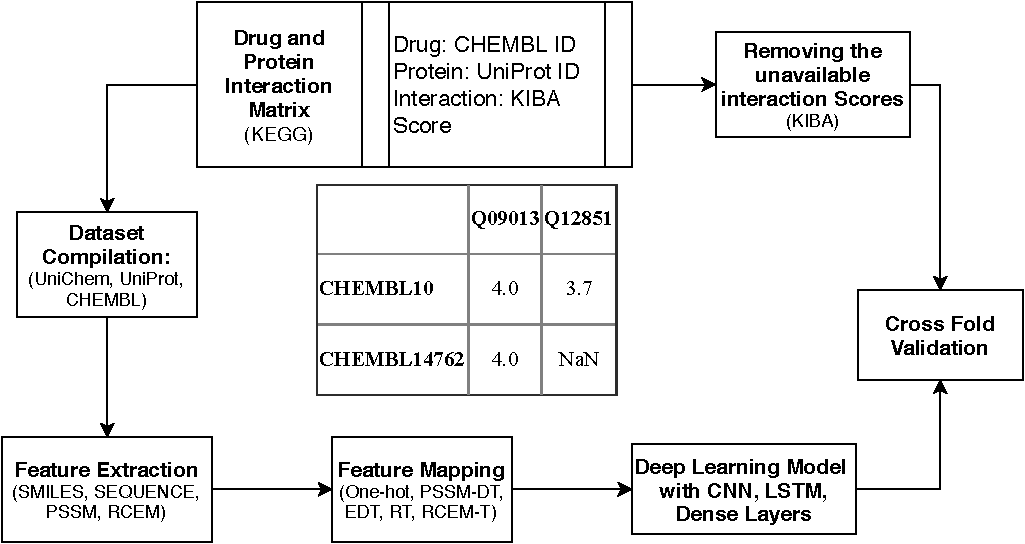
\includegraphics[width=1\linewidth]{mainmatter/3-Methodology/images/block.pdf}
\caption{System Block Diagram}
\label{fig:system}
\end{figure}

The Figure ~\ref{fig:system} shows the various components used to form the prediction system. The idea is basic in that protein interaction depends on the structural and chemical properties. The structural components are fulfilled and


\section{Dataset}

\subsection{KEGG}
It is a community-driven database which holds large-scale molecular datasets generated by genome sequencing and high-throughput experimental techniuqe.\cite{Kanehisa2000} We use \acrshort{kegg} DRUG dataset for finding the interaction set between DRUG and PROTEIN. The interaction score is based on Equation ~\ref{eq:kiba}:
% \begin{flushright}
\begin{equation}[ht]
  KIBA = \begin{cases}
    K_i . {adj} & \quad {if} \; {IC_{50}\: and\, K_i \,are\, present} \\
    K_b.{adj} & \quad {if}  {IC_{50} \, and \, K_d \, are \, present} \\
    \frac{K_i . {adj} \; K_b.{adj}}{2} & \quad {if\, IC_{50}\,,K_i\, and \,K_d\, are\, present}
  \end{cases}
   \label{eq:kiba}
\end{equation}
where L\textsubscript{d} and L\textsubscript{i} are parameters defining weights of IC\textsubscript{50} in model adjustments for K\textsubscript{i} and K\textsubscript{b} 
% \end{flushright}

For a kinase inhibitor drug−target interaction, we consider the medians of three major bioactivity types IC\textsubscript{50}, K\textsubscript{i}, K\textsubscript{d} where
IC\textsubscript{50} \cite{Tang2013} is the concentration at which the inhibitor causes a 50\% inhibition of enzymatic activity and K\textsubscript{i} is defined by \begin{equation}
    Ki = \frac{IC_{50}} {1 + [S]  K_m}
    \label{eq:ki}
\end{equation} 
where,  [{S}] is the experimental substrate concentration and K\textsubscript{m} is the concentration of the substrate.

\iffalse
\begin{equation}
    \tau= \frac{(a−b)}{n(n − 1)/2}   
    \label{eq:tau}
  \end{equation}
  { Here {a} and {b} represent the number of concordant pairs and discordant pairs respectively. }
\fi



\begin{equation}
K_i.{adj} = \frac{IC_{50}}{1 + L_i(IC_{50}/K_i)}
\label{eq:ki_adj}
\end{equation}

\begin{equation}
K_d.{adj} = \frac{IC_{50}}{1 + L_d(IC_{50}/K_d)}
\end{equation}

All the bioactivity types are available from CHEMBL.\cite{Gaulton2017} We thus have 254 proteins and 52498 drugs. Based on interaction data available, we remove the unknown values and get a total of 180244 interaction KIBA score values in the range of -3.09 to 17.8. With the standard deviation of 1.22, we try to predict the best KIBA score of drug and protein based on the sequence information alone.
\begin{figure}
  \centering 
        %  \subfloat[]{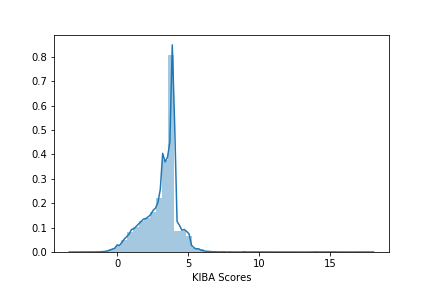
\includegraphics[width=.3\textwidth]{mainmatter/3-Methodology/images/data/distribution.png}}
         \subfigure[KIBA Scores]{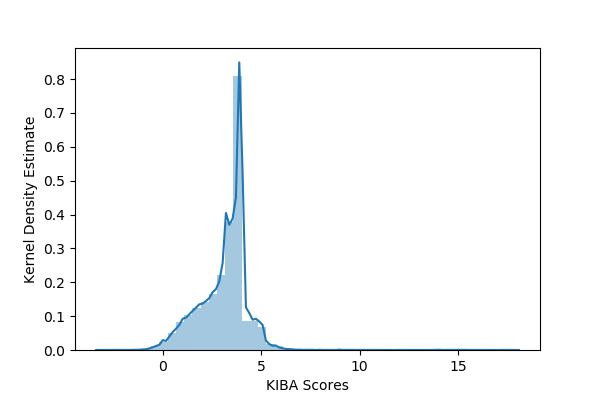
\includegraphics[width=.7\textwidth]{mainmatter/3-Methodology/images/figures/distribution.png}}
         \subfigure[Logarithmic One Hot Encodings of Drug Sequence]{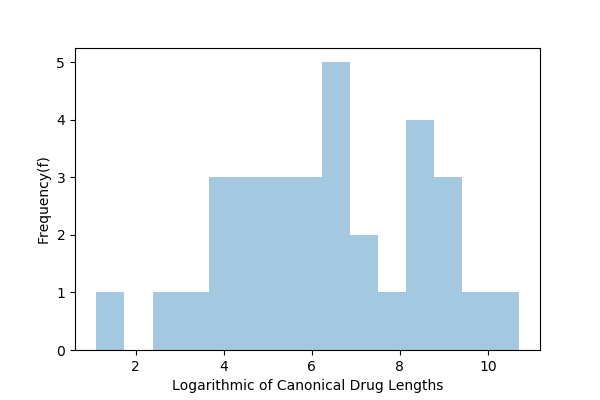
\includegraphics[width=.7\textwidth]{mainmatter/3-Methodology/images/figures/drug_length_logarithmic.png}}
         \subfigure[One Hot Encodings of Protein Sequence]{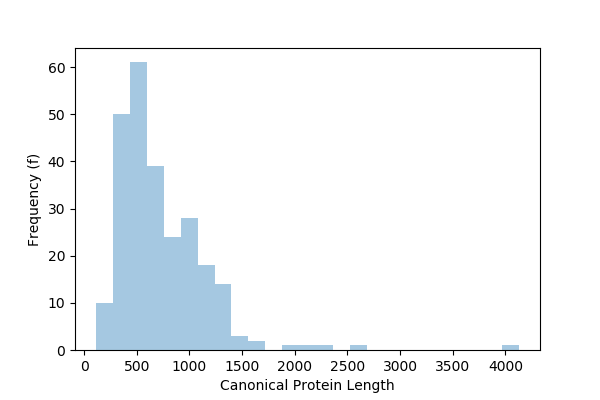
\includegraphics[width=.7\textwidth]{mainmatter/3-Methodology/images/figures/prot_length.png}}
         \caption{Data Distribution of KIBA-interaction scores, Drug Sequences and Protein Sequences}
         \label{fig:kiba_drug_protein}
\end{figure}

\subsection{UniProt and CHEMBL }

\subsubsection{UniProt} 
The sequence related information of protein is referenced using UniProt Identifier and protein sequence (FASTA) is called using the api from UniProt. \cite{UniProtConsortium2018}


\subsubsection{CHEMBL}
The molecular fingerprints related to drugs are referenced usning CHEMBL Identifier and the drug sequence is called from CHEMBL database. \cite{Gaulton2017}

\subsection{PSI-BLAST}
It relates with multiple sequence alignments from a family of protein sequences\cite{Schaffer2001}. This helps us to create a \acrshort{pssm} - Equation (\ref{eq:pssm}) - matrix referred to as secondary protein structure. The improvement in drug-contact prediction can be thought for amino acid composition being tuned with the scoring system. For this study, the PSSM profile of every protein sequence is obtained by executing iteration of PSI-BLAST against \cite[KEGG]{Schaffer2001} protein. PSSM profile is a matrix of L*20 dimensions where, 20 referring to standard type of amino acids and L being the length of the protein. The larger positive scores represent conserved positions, which in turn implies critical functional residues that are required to perform various intermolecular interactions.\cite[PSSM]{Schaffer2001}

\begin{equation}
  PSSM = \begin{bmatrix}
    P_{1,1} & P_{1,2} & \dots & P_{1,20} \\
    P_{2,1} & P_{2,2} & \dots & P_{2,20} \\
    \vdots  & \vdots  & \ddots & \vdots \\
    P_{2,1} & P_{2,2} & \dots & P_{2,20} \\
  \end{bmatrix}
  \label{eq:pssm}
\end{equation}

\subsubsection{PSSM-DT}
Two forms of \acrshort{pssm} distance transformation techniques are used to transform the \acrshort{pssm} information into fixed dimensional vectors \cite{Xu2015}. The PSSM-DT (PSSM-Distance Transformation) can transform the \acrshort{pssm} information into uniform numeric representation by approximately measuring the occurrence probabilities of any pairs of amino acid. It results in two types of feature matrices: PSSM-SDT and PSSM-DDT defined by:

\begin{equation}
  PSSM-SDT(i,lg) = \sum_{i=1}^{L-lg} S_{i,j} \times \frac{ S_{i,j+lg} }{L-lg} 
  \label{eq:pssmsdt}
\end{equation}
\textit{\center lg =  distance of separation between same amino acid sequence}

\begin{equation}
  PSSM-DDT(i_1,i_2, lg) = \sum_{j=1}^{L-lg} S_{i_1,j} \times \frac{ S_{i_2,j+lg} }{ L-lg} 
  \label{eq:pssmddt}
\end{equation}
\textit{\centering i\textsubscript{1} and i\textsubscript{2} refer to tow different types of amino acids}

Thus we have [380 ~\eqref{eq:pssmddt}+20 ~\eqref{eq:pssmsdt} = 400] x lg matrix which will be used as protein-specific vector in this work.

\subsubsection{Evolutionary Distance Transformation Matrix}
The mutational information of protein can be more informative than the sequence information itself\cite{Zhang2014}. Evolutionary difference formula(EDF) is used to represent mutation difference between adjacent residues. Secondly, the PSSM is converted into 20 x 20 matrix (ED-PSSM). This extracts the non co-occurrence probability for two amino acids separated by a certain distance \textit{d} in the protein from the PSSM profile. For example, d=1 implies that the two amino acids are consecutive; d=2 implies that there is one amino acid between the two. Then the EDT feature vector computed from ED-PSSM can be represented as (~\ref{eq:Pmat}): 
\begin{equation}
  \label{eq:Pmat}
  P = [ \partial_1 ,\partial_2, \dots, \partial_\Omega]
\end{equation}
where $\Omega$ is an integer that represents the dimension of the vector whose value is 400.. The non-co-occurrence probability of two amino acids separated by distance \textit{d} can be computed as:
\begin{equation}
  f(A_x,A_y) = \sum_{d=1}^{D} \frac{1}{L-d} \sum_{i=1}^{L-d} (P_{i,x} - P_{i+d,y})^2
  \label{eq:edt}
\end{equation}
where $P_{i,x}$ and $P_{i+d,y}$ are the elements in the PSSM profile; $A_x$ and $A_y$ represent any of the the 20 different amino acids in the protein sequence. Finally we spread the $f(A_x,A_y)$ in equation ~\ref{eq:Pmat} as:
$ \partial_1 = f(A_1,A_2) $, 
$ \partial_{400} = f(A_20, A_20) $


\subsection{Residue feature} 
The Statistical Residue Vector Space \acrshort{srv} \cite{Wong2018} plays an important role in Residue Residue Interaction and thus creates a basis for structural stability of the protein sequence itself. Though related more to the tertiary structure of protein sequence itself, we regard it to create a correlated sequence information where two proteins are related distantly by sequence but highly related with functional characteristic of protein. Table ~\ref{table:r2r} shows the table used in this work. It is a 20 x 20 matrix whose rows and columns represent 20 standard amino acids.

\subsubsection{Residue Probing Transformation(RPT) feature}
RPT as proposed by \cite[{Jeong et al.}]{Jeong2011}, and implemented by \cite[Pujan et al.]{Mishra2019}, emphasizes domains with similar conservation rates by grouping domain families based on their conservation score in the PSSM profile.
\begin{equation}
  RPT = \begin{bmatrix}
    H_{1,1} & H_{1,2} & \dots & H_{1,20} \\
    H_{2,1} & H_{2,2} & \dots & H_{2,20} \\
    \vdots  & \vdots  & \ddots & \vdots \\
    H_{2,1} & H_{2,2} & \dots & H_{2,20} \\
  \end{bmatrix}
  \label{eq:rpt}
\end{equation}
The RPT matrix (Equation ~\ref{eq:rpt}) is then tranformed into feature vector of 400 dimensions, as shown in Equation ~\ref{eq:rptV}.

\begin{equation}
  V = [ f_{s_{1,1}}, f_{s_{1,2}}, \dots, f_{s_{i,j}}, \dots, f_{s_{20,20}} ]
  \label{eq:rptV}
\end{equation}
where, 
\begin{equation}
  f_{s_{i,j}} = \frac{s_{i,j}}{L} (i,j = 1,2,\dots,20)
  \label{eq:rptF}
\end{equation}


\section{Deep Learning Model}

The Features thus formed are then subjected to deep learning model using keras library in python. We use the Embedding feature provided by keras as other features for both drug fingerprint and protein sequence. The implemented model is represented by Figure ~\ref{fig:dlm}. The input layers are described in Table ~\ref{table:inputs}.

\begin{figure}[ht]
\centering
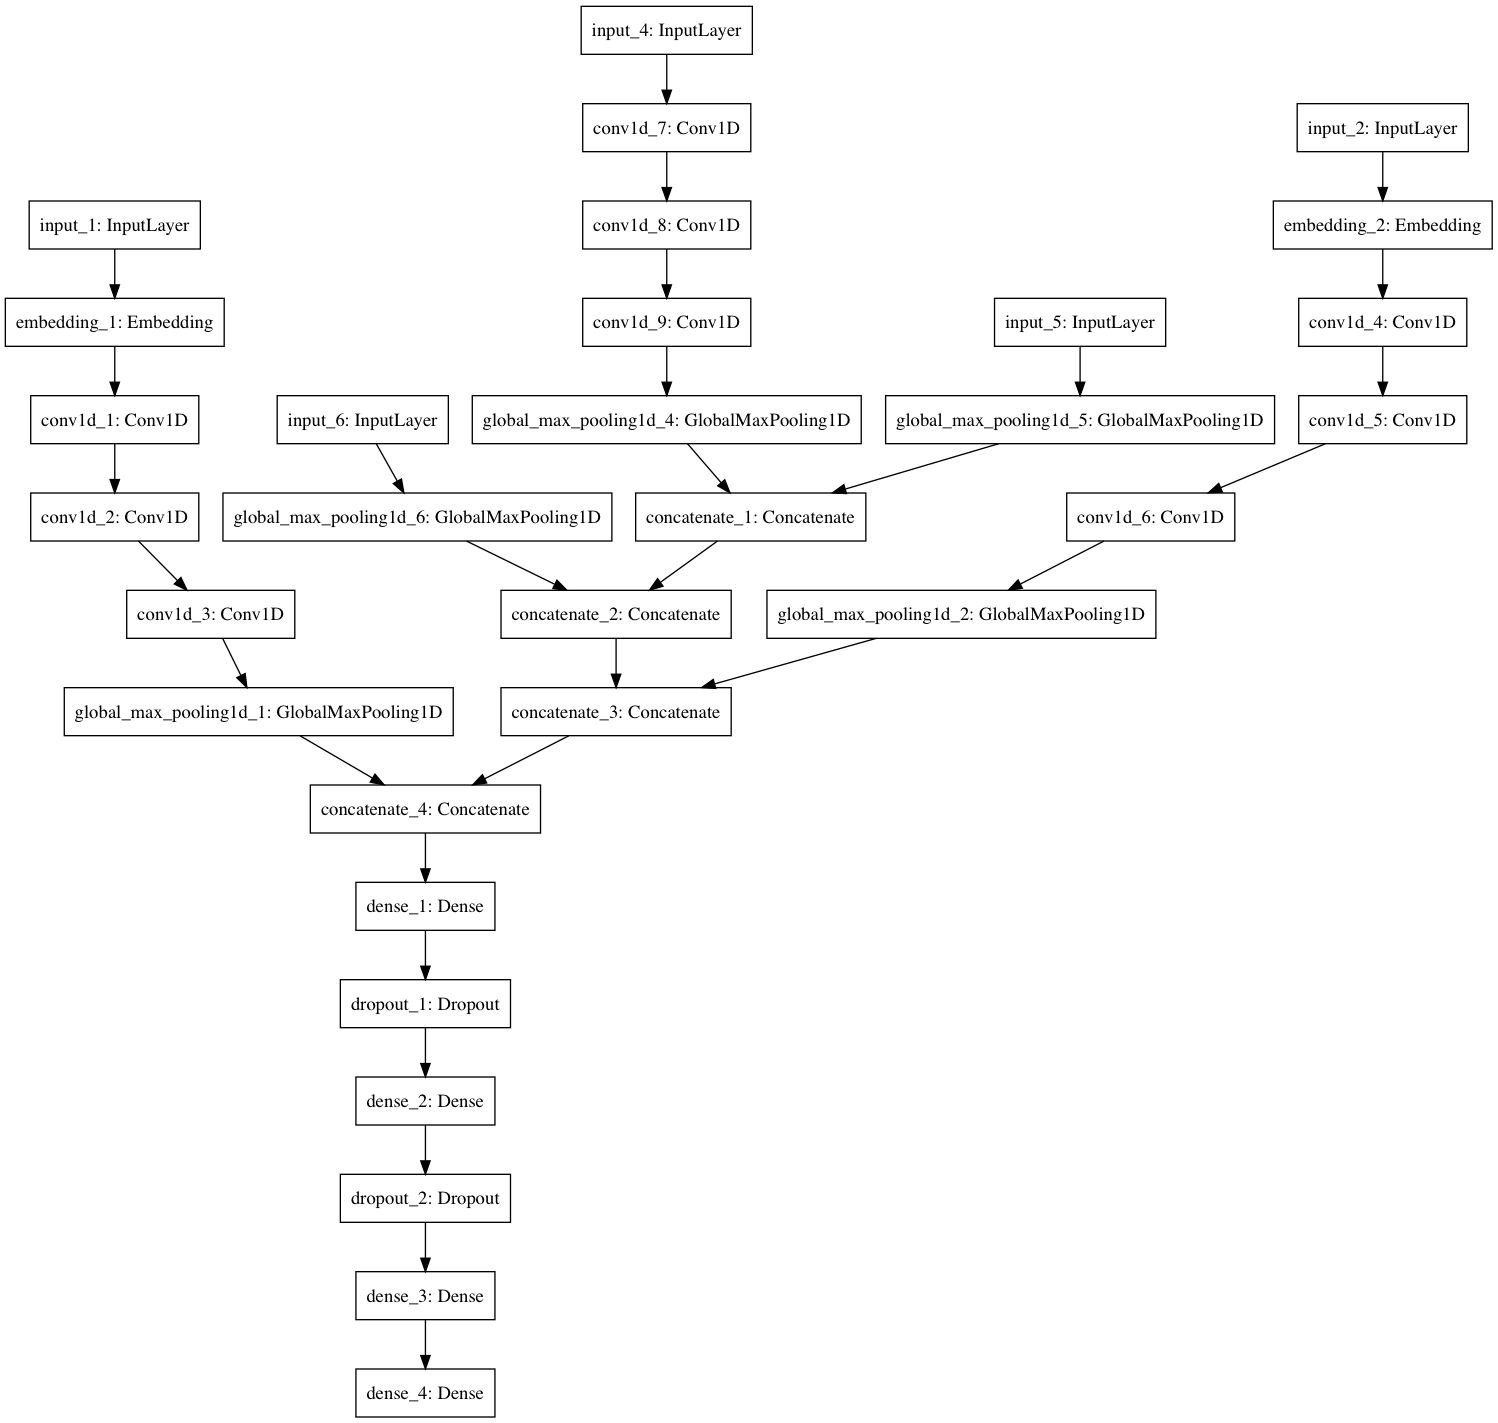
\includegraphics[width=1\linewidth]{mainmatter/3-Methodology/images/build_combined_categorical_tensor_contact_new.png}
\caption{Deep Learning Model}
\label{fig:dlm}
\end{figure}
\begin{table}[ht]\centering
  \begin{tabular}{|l|l|l|l|}
    
    \hline \label{table:inputs}
    S.No. & Input Layer Name & Used Feature Vector & Type \\ \hline
    1 & input\_1 & One Hot Encoding & Drug \\ \hline
    2 & input\_2 & One Hot Encoding & Protein \\ \hline
    3 & input\_3 & Evolutionary Distance Transformation Vector& Protein \\ \hline
    4 & input\_4 & PSSM-DT Vector & Protein \\ \hline
    5 & input\_5 & Residue Probing Transformation Vector & Protein \\   \hline 
  \end{tabular} 
  \caption{Inputs Used in the Deep Learning Network} 
\end{table}

\subsection{Components description used from Tensorflow (Keras)}
\subsubsection{Embedding Layer}
The one-hot encodings of the drugs and protein sequences are inputs to this layer. It turns positive integers (indexes) into dense vectors of fixed size. eg. [[4], [20]] -> [[0.25, 0.1], [0.6, -0.2]].

\subsubsection{Dense Layer}
It is a neural layer which fully connects the input layer to output layer. It can be seen from Figure ~\ref{fig:dense}.
\begin{figure}[ht]
  \centering
  % 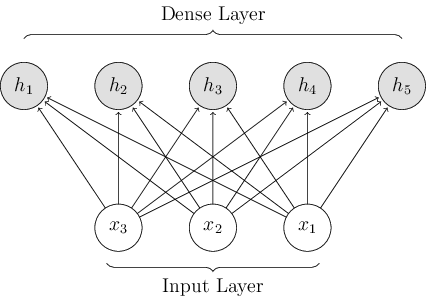
\includegraphics[width=.5\linewidth]{mainmatter/3-Methodology/images/dense.png}
  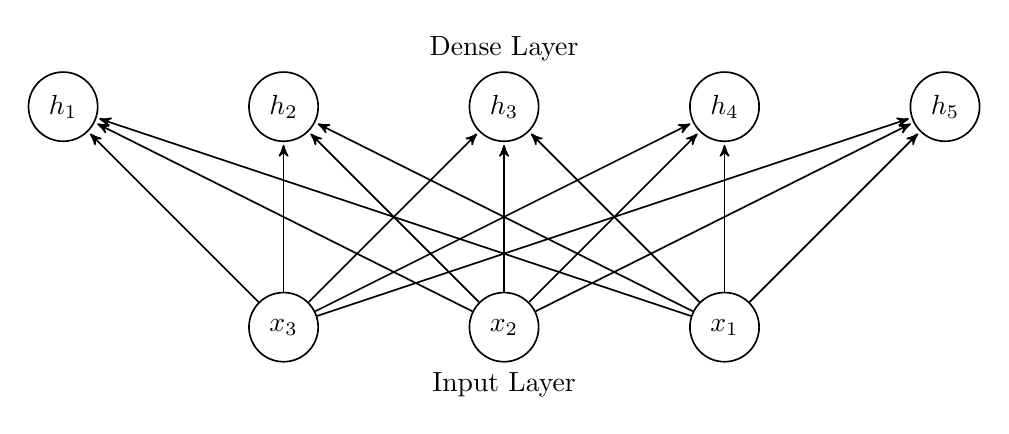
\begin{tikzpicture}[->,>=stealth',shorten >=1pt,auto,node distance=2.8cm,
    semithick]

      \tikzstyle{every state}=[text=black]
      \node[state]          (A)   {$h_1$};
      \node[state]         (B)  [right of=A] {$h_2$};
      \node[label=above:{Dense Layer},state]         (C) [right of=B] {$h_3$} ;
      \node[state]         (D) [right of=C] {$h_4$};
      \node[state]         (E) [right of=D] {$h_5$};

      \node[state]         (X1) [below of=B] {$x_3$};
      \node[state, label=below:{Input Layer}]         (X2) [right of=X1]       {$x_2$};
      \node[state]         (X3) [right of=X2]       {$x_1$};

      \path (X1) 
      edge              node {} (A)
      edge              node {} (B)
      edge              node {} (C)
      edge              node {} (D)
      edge              node {} (E)
      % edge              node {1,1,R} (C)
      (X2) 
      edge              node {} (A)
      edge              node {} (B)
      edge              node {} (C)
      edge              node {} (D)
      edge              node {} (E)
      % edge              node {0,1,L} (C)
      (X3)
      edge              node {} (A)
      edge              node {} (B)
      edge              node {} (C)
      edge              node {} (D)
      edge              node {} (E);
      % edge [bend left]  node {1,0,R} (E);

\end{tikzpicture}

  \caption{Dense Layer}
  \label{fig:dense}
\end{figure}

\subsubsection{Dropout Layer}
It is undesirable when every component of the input layer makes a significant changes to the output layer. To reduce the effect of unimportant features we use dropout layer. Thus the backpropagation network tries to ignore the noise features and minimizes the unrealizable prediction of the learning problem. This can be expressed diagrammatically in the Figure ~\ref{fig:dropout}.
\begin{figure}
  [ht] \centering
  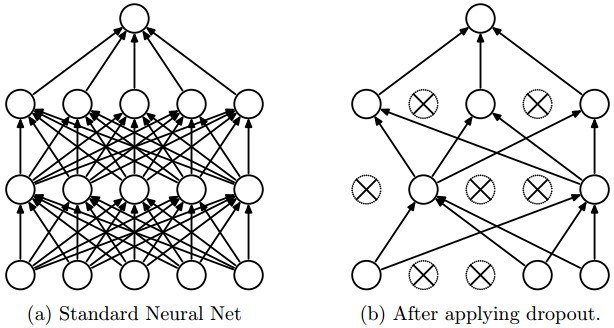
\includegraphics[width=.5\linewidth]{mainmatter/3-Methodology/images/dropout.jpeg}
  \caption{Dropout Layer}
  \label{fig:dropout}

\end{figure}

\subsubsection{Global Max Pooling Layer}
We use this to sample the learned parameters from the grid of 3 dimensions returned by Convolution Layer. It gets reduced to 1 dimension by taking the highest values from the window size(corresponding to shape of 1\textsuperscript{st} dimensional element).
\begin{figure}
  [ht]\centering
  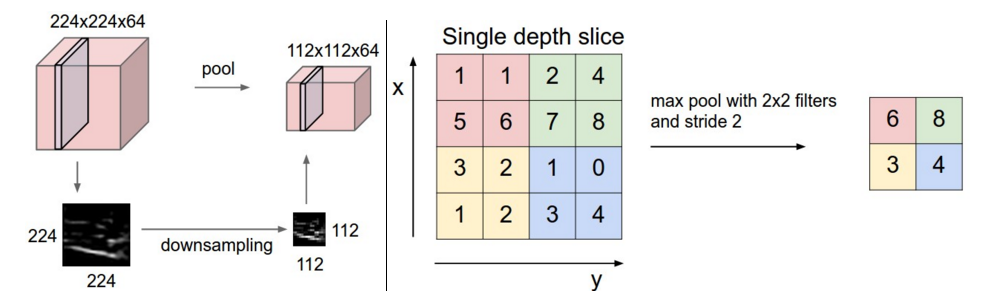
\includegraphics[width=.75\linewidth]{mainmatter/3-Methodology/images/pooling.png}
  \caption{Pooling Layer}
  \label{fig:pool_layer}
\end{figure}

\subsubsection{Concatenation Layer}
It is used to simply join two vectors so that we create a feature set comprising of multiple features whose positional index indicates the feature set being manipulated.

\subsubsection{Convolution Neural Network}
To learn the local patterns in the input vector, we use \acrshort{cnn}. While Dense Layers and \acrshort{lstm} learn the global patterns, \acrshort{cnn} is used to understand the local patterns. It does so by increasing the depth layer, which in turn is designed to learn different patterns as shown in Figure ~\ref{fig:cnn}.
\begin{figure}[ht]
  \centering
  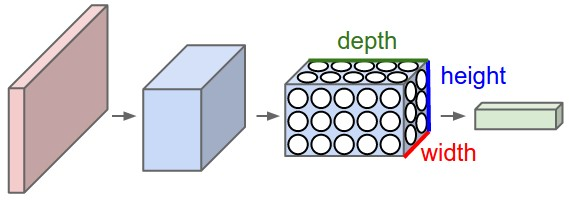
\includegraphics[width=.5\linewidth]{mainmatter/3-Methodology/images/cnn.jpg}
  \caption{Convolutional Neural Network}
  \label{fig:cnn}
\end{figure}

\subsubsection{LSTM}
As the RNN often suffers from vanishing gradient problem, we use a \acrshort{lstm} Layer to learn the global pattern of the feature sets resulting after concatenation of different stacked layers outputs. The LSTM architecture can be seen in figure below:
\begin{figure}
  [ht]
  \centering
  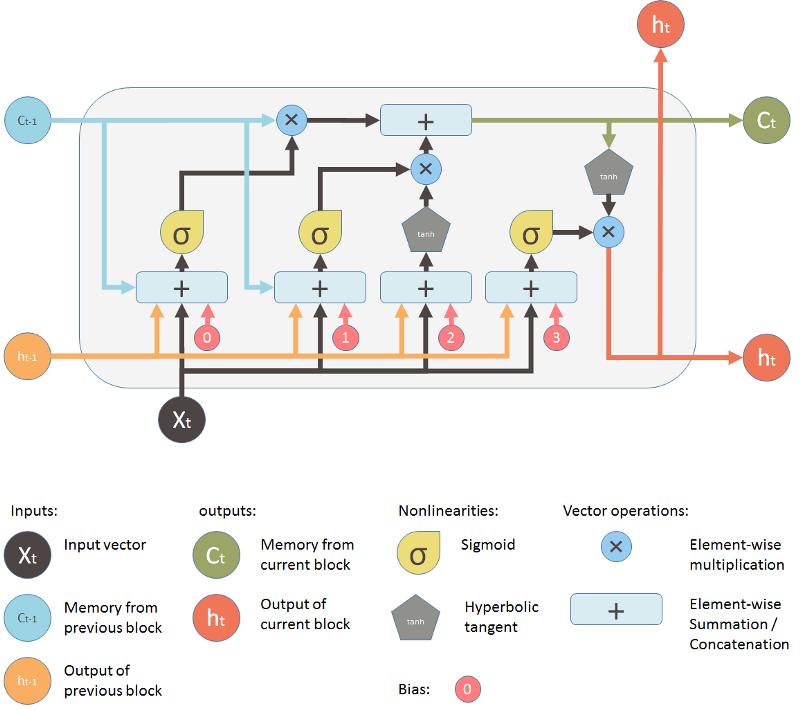
\includegraphics[width=.5\linewidth]{mainmatter/3-Methodology/images/LSTMBlockDiagram.png}
  \caption{Long Short Term Memory}
  \label{fig:lstm}
\end{figure}



